\documentclass[a4paper,11pt]{article}


\usepackage{amsmath,amsfonts,amsthm,a4wide}
\usepackage{graphicx}
\usepackage[super]{nth}
\usepackage{mathtools}


\begin{document}
\begin{center}
University of Toronto at Scarborough\\[0.1in]
{\bf CSCC73H3 Algorithm Design and Analysis, FALL 2018} \\[0.1in]
{\large{\bf Assignment No.4: Dynamic Programming}}\\[0.1in]
{\bf DUE:} October 24, 2018, at 11:59 pm
\end{center}


\vspace{0.1in}
\noindent
{\bf Student ID:} 1005642654 \\[0.15in]
{\bf Student Name:} KyooSik Lee
\vspace{0.3in}

\vspace{0.3in}
\begin{enumerate}

\item {\bf Description}

My algorithm uses Bellman-Ford algorithm with a slight change. Instead of adding the values, my algorithm will multiply the value of edge rate cost while on the iterations for Bellman-Ford algorithm. When filling up the table for Bellman-Ford algorithm, the algorithm will only update when the calculated ratio is bigger, which is different to the original Bellman-Ford algorithm. We will call this Modified-Bellman-Ford algorithm.

For given graph $G$, add one vertex $t$ which we will make to be a sink vertex. Then add edges from every vertices to $t$. The augmented graph $G'$follows(All the red edges pointing at $t$ has cost rate of 1).


\begin{figure}[hbt]
	\centering
	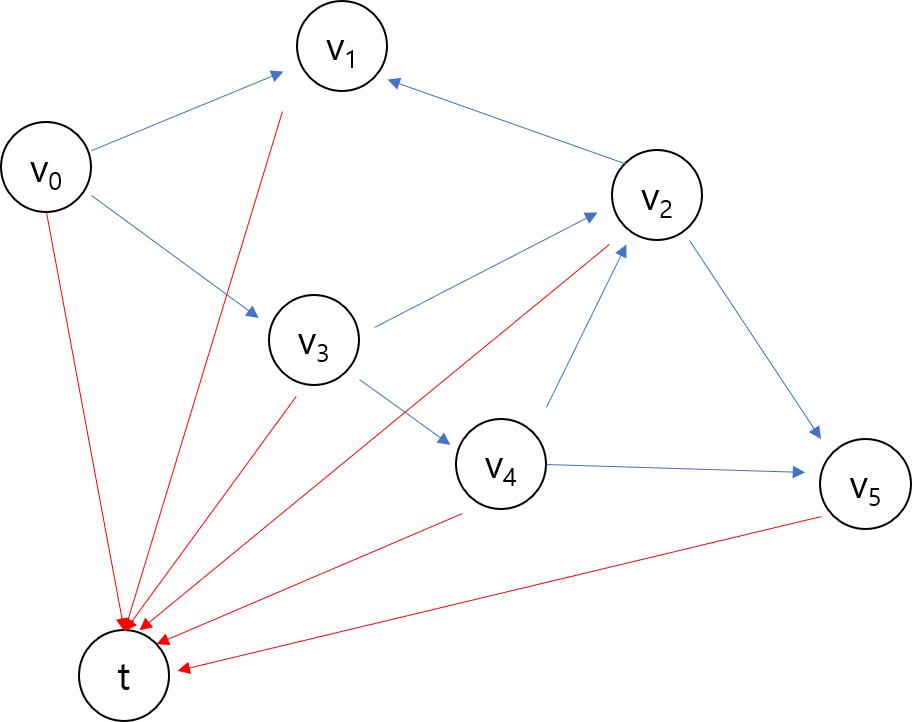
\includegraphics[scale=0.5]{figure3.png}
	\caption{Augmented Graph $G'$}
\end{figure}

Then do the Modified-Bellman-Ford algorithm with destination set to $t$.

If $G'$ has {\it profitable cycle}, then the original graph $G$ has {\it profitable cycle}. This is because the sink vertex $t$ has no out-edge, which means that the {\it profitable cycle} must be in original graph $G$.

Finding {\it profitable cycle} is done by conducting extra iteration on the original Bellman-Ford algorithm. 
Note that original algorithm has $n-1$ iteration.
After the $n^{th}$ iteration, if the value on the table changes, then $G'$ has {\it profitable cycle} and therefore $G$ has {\it profitable cycle}. 
Tracing could be easily handled by an array that holds pointer to the next vertex everytime that vertex has updated. 
This array is called pointer array. 
By examining pointer array starting from the vertex that changed after $n^{th}$ iteration, we can trace the vertices on the {\it profitable cycle}. If there is a vertex that appears twice, the path between them is the {\it profitable cycle}.

{\bf Complexity}

Complexity is same as original Bellman-Ford algorithm. It is $O(mn)$ where $m$ is the number of edges and $n$ is the number of vertices.


\item 

{\bf Description}

Use the method of Bellman-Ford algorithm, but slightly different way. Note that the graph has no negative cycle so Bellman-Ford algorithm works well. But this time, store another value indicating the number of shortest path like following example graph and table.
\begin{figure}[hbt]
	\centering
	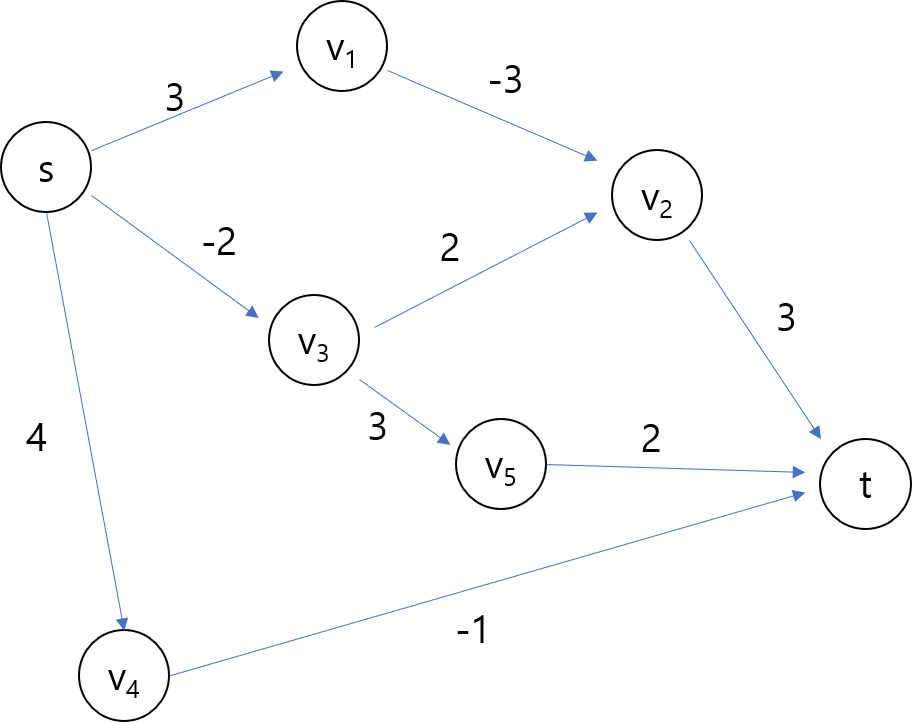
\includegraphics[scale=0.5]{figure2.png}
	\caption{Example Graph}
\end{figure}

\begin{center}
\begin{tabular}{lllllll}
                       & 0                         & 1                     & 2                     & 3                     & 4                     & 5                     \\ \cline{2-7} 
\multicolumn{1}{l|}{t} & \multicolumn{1}{l|}{(0,1)} & \multicolumn{1}{l|}{...} & \multicolumn{1}{l|}{...} & \multicolumn{1}{l|}{...} & \multicolumn{1}{l|}{...} & \multicolumn{1}{l|}{...} \\ \cline{2-7} 
\multicolumn{1}{l|}{s} & \multicolumn{1}{l|}{($\infty$,0)} & \multicolumn{1}{l|}{...} & \multicolumn{1}{l|}{...} & \multicolumn{1}{l|}{...} & \multicolumn{1}{l|}{...} & \multicolumn{1}{l|}{...} \\ \cline{2-7} 
\multicolumn{1}{l|}{$v_1$} & \multicolumn{1}{l|}{($\infty$,0)} & \multicolumn{1}{l|}{...} & \multicolumn{1}{l|}{...} & \multicolumn{1}{l|}{...} & \multicolumn{1}{l|}{...} & \multicolumn{1}{l|}{...} \\ \cline{2-7} 
\multicolumn{1}{l|}{$v_2$} & \multicolumn{1}{l|}{($\infty$,0)} & \multicolumn{1}{l|}{...} & \multicolumn{1}{l|}{...} & \multicolumn{1}{l|}{...} & \multicolumn{1}{l|}{...} & \multicolumn{1}{l|}{...} \\ \cline{2-7} 
\multicolumn{1}{l|}{$v_3$} & \multicolumn{1}{l|}{($\infty$,0)} & \multicolumn{1}{l|}{...} & \multicolumn{1}{l|}{...} & \multicolumn{1}{l|}{...} & \multicolumn{1}{l|}{...} & \multicolumn{1}{l|}{...} \\ \cline{2-7} 
\multicolumn{1}{l|}{$v_4$} & \multicolumn{1}{l|}{($\infty$,0)} & \multicolumn{1}{l|}{...} & \multicolumn{1}{l|}{...} & \multicolumn{1}{l|}{...} & \multicolumn{1}{l|}{...} & \multicolumn{1}{l|}{...} \\ \cline{2-7} 
\multicolumn{1}{l|}{$v_5$} & \multicolumn{1}{l|}{($\infty$,0)} & \multicolumn{1}{l|}{...} & \multicolumn{1}{l|}{...} & \multicolumn{1}{l|}{...} & \multicolumn{1}{l|}{...} & \multicolumn{1}{l|}{...} \\ \cline{2-7} 
\end{tabular}
\end{center}

Everytime a shortest path is updated initially, it should have the indicator as 1 because it has only one edge. So the following table is the result after the first iteration.

\begin{center}
\begin{tabular}{lllllll}
                       & 0                         & 1                     & 2                     & 3                     & 4                     & 5                     \\ \cline{2-7} 
\multicolumn{1}{l|}{t} & \multicolumn{1}{l|}{(0,1)} & \multicolumn{1}{l|}{(0,1)} & \multicolumn{1}{l|}{...} & \multicolumn{1}{l|}{...} & \multicolumn{1}{l|}{...} & \multicolumn{1}{l|}{...} \\ \cline{2-7} 
\multicolumn{1}{l|}{s} & \multicolumn{1}{l|}{($\infty$,0)} & \multicolumn{1}{l|}{($\infty$,0)} & \multicolumn{1}{l|}{...} & \multicolumn{1}{l|}{...} & \multicolumn{1}{l|}{...} & \multicolumn{1}{l|}{...} \\ \cline{2-7} 
\multicolumn{1}{l|}{$v_1$} & \multicolumn{1}{l|}{($\infty$,0)} & \multicolumn{1}{l|}{($\infty$,0)} & \multicolumn{1}{l|}{...} & \multicolumn{1}{l|}{...} & \multicolumn{1}{l|}{...} & \multicolumn{1}{l|}{...} \\ \cline{2-7} 
\multicolumn{1}{l|}{$v_2$} & \multicolumn{1}{l|}{($\infty$,0)} & \multicolumn{1}{l|}{(3,1)} & \multicolumn{1}{l|}{...} & \multicolumn{1}{l|}{...} & \multicolumn{1}{l|}{...} & \multicolumn{1}{l|}{...} \\ \cline{2-7} 
\multicolumn{1}{l|}{$v_3$} & \multicolumn{1}{l|}{($\infty$,0)} & \multicolumn{1}{l|}{($\infty$,0)} & \multicolumn{1}{l|}{...} & \multicolumn{1}{l|}{...} & \multicolumn{1}{l|}{...} & \multicolumn{1}{l|}{...} \\ \cline{2-7} 
\multicolumn{1}{l|}{$v_4$} & \multicolumn{1}{l|}{($\infty$,0)} & \multicolumn{1}{l|}{(-1,1)} & \multicolumn{1}{l|}{...} & \multicolumn{1}{l|}{...} & \multicolumn{1}{l|}{...} & \multicolumn{1}{l|}{...} \\ \cline{2-7}  
\multicolumn{1}{l|}{$v_5$} & \multicolumn{1}{l|}{($\infty$,0)} & \multicolumn{1}{l|}{(2,1)} & \multicolumn{1}{l|}{...} & \multicolumn{1}{l|}{...} & \multicolumn{1}{l|}{...} & \multicolumn{1}{l|}{...} \\ \cline{2-7} 
\end{tabular}
\end{center}

And whenever the length value is updated, change the indicator of the wll-be-updated vertex to the indicator of next vertex's indicator.

When there is a tie, change the indicator of the will-be-updated vertex by adding the indicator of next vertex's indicator.

After some iteration the table will look like following.

\begin{center}
\begin{tabular}{lllllll}
                       & 0                         & 1                     & 2                     & 3                     & 4                     & 5                     \\ \cline{2-7} 
\multicolumn{1}{l|}{t} & \multicolumn{1}{l|}{(0,1)} & \multicolumn{1}{l|}{(0,1)} & \multicolumn{1}{l|}{(0,1)} & \multicolumn{1}{l|}{...} & \multicolumn{1}{l|}{...} & \multicolumn{1}{l|}{...} \\ \cline{2-7} 
\multicolumn{1}{l|}{s} & \multicolumn{1}{l|}{($\infty$,0)} & \multicolumn{1}{l|}{($\infty$,0)} & \multicolumn{1}{l|}{(3,1)} & \multicolumn{1}{l|}{...} & \multicolumn{1}{l|}{...} & \multicolumn{1}{l|}{...} \\ \cline{2-7} 
\multicolumn{1}{l|}{$v_1$} & \multicolumn{1}{l|}{($\infty$,0)} & \multicolumn{1}{l|}{($\infty$,0)} & \multicolumn{1}{l|}{(0,1)} & \multicolumn{1}{l|}{...} & \multicolumn{1}{l|}{...} & \multicolumn{1}{l|}{...} \\ \cline{2-7} 
\multicolumn{1}{l|}{$v_2$} & \multicolumn{1}{l|}{($\infty$,0)} & \multicolumn{1}{l|}{(3,1)} & \multicolumn{1}{l|}{(3,1)} & \multicolumn{1}{l|}{...} & \multicolumn{1}{l|}{...} & \multicolumn{1}{l|}{...} \\ \cline{2-7} 
\multicolumn{1}{l|}{$v_3$} & \multicolumn{1}{l|}{($\infty$,0)} & \multicolumn{1}{l|}{($\infty$,0)} & \multicolumn{1}{l|}{(5,2)} & \multicolumn{1}{l|}{...} & \multicolumn{1}{l|}{...} & \multicolumn{1}{l|}{...} \\ \cline{2-7} 
\multicolumn{1}{l|}{$v_4$} & \multicolumn{1}{l|}{($\infty$,0)} & \multicolumn{1}{l|}{(-1,1)} & \multicolumn{1}{l|}{(-1,1)} & \multicolumn{1}{l|}{...} & \multicolumn{1}{l|}{...} & \multicolumn{1}{l|}{...} \\ \cline{2-7}  
\multicolumn{1}{l|}{$v_5$} & \multicolumn{1}{l|}{($\infty$,0)} & \multicolumn{1}{l|}{(2,1)} & \multicolumn{1}{l|}{(2,1)} & \multicolumn{1}{l|}{...} & \multicolumn{1}{l|}{...} & \multicolumn{1}{l|}{...} \\ \cline{2-7} 
\end{tabular}
\end{center}

At this time, it is only worth looking at the $s,v_1,v_3$ because the value has updated. For $s$, there is no invertex so there is nothing to do. For $v_1$, it has a edge from $s$ to $v_1$. Therefore we have to compare the value of $M(s,2)$ with $edgecost(s, v_1)+ M(v_1,2)$ which is a tie. therefore we add $v_1$'s indicator to the s value so resulting table will be the table following.

\begin{center}
\begin{tabular}{lllllll}
                       & 0                         & 1                     & 2                     & 3                     & 4                     & 5                     \\ \cline{2-7} 
\multicolumn{1}{l|}{t} & \multicolumn{1}{l|}{(0,1)} & \multicolumn{1}{l|}{(0,1)} & \multicolumn{1}{l|}{(0,1)} & \multicolumn{1}{l|}{...} & \multicolumn{1}{l|}{...} & \multicolumn{1}{l|}{...} \\ \cline{2-7} 
\multicolumn{1}{l|}{s} & \multicolumn{1}{l|}{($\infty$,0)} & \multicolumn{1}{l|}{($\infty$,0)} & \multicolumn{1}{l|}{(3,1)} & \multicolumn{1}{l|}{(3,2)} & \multicolumn{1}{l|}{...} & \multicolumn{1}{l|}{...} \\ \cline{2-7} 
\multicolumn{1}{l|}{$v_1$} & \multicolumn{1}{l|}{($\infty$,0)} & \multicolumn{1}{l|}{($\infty$,0)} & \multicolumn{1}{l|}{(0,1)} & \multicolumn{1}{l|}{...} & \multicolumn{1}{l|}{...} & \multicolumn{1}{l|}{...} \\ \cline{2-7} 
\multicolumn{1}{l|}{$v_2$} & \multicolumn{1}{l|}{($\infty$,0)} & \multicolumn{1}{l|}{(3,1)} & \multicolumn{1}{l|}{(3,1)} & \multicolumn{1}{l|}{...} & \multicolumn{1}{l|}{...} & \multicolumn{1}{l|}{...} \\ \cline{2-7} 
\multicolumn{1}{l|}{$v_3$} & \multicolumn{1}{l|}{($\infty$,0)} & \multicolumn{1}{l|}{($\infty$,0)} & \multicolumn{1}{l|}{(5,2)} & \multicolumn{1}{l|}{...} & \multicolumn{1}{l|}{...} & \multicolumn{1}{l|}{...} \\ \cline{2-7} 
\multicolumn{1}{l|}{$v_4$} & \multicolumn{1}{l|}{($\infty$,0)} & \multicolumn{1}{l|}{(-1,1)} & \multicolumn{1}{l|}{(-1,1)} & \multicolumn{1}{l|}{...} & \multicolumn{1}{l|}{...} & \multicolumn{1}{l|}{...} \\ \cline{2-7}  
\multicolumn{1}{l|}{$v_5$} & \multicolumn{1}{l|}{($\infty$,0)} & \multicolumn{1}{l|}{(2,1)} & \multicolumn{1}{l|}{(2,1)} & \multicolumn{1}{l|}{...} & \multicolumn{1}{l|}{...} & \multicolumn{1}{l|}{...} \\ \cline{2-7} 
\end{tabular}
\end{center}

Now, we have to check $v_3$. It has incoming edge from s. So we have to check $M(s,3)$(now that it is up in the table) with $edgecost(s,v_3)+M(v_3,2)$ which is a tie. Therefore we have to add $M(v_3,2)$'s indicator to $M(s,3)$'s indicator resulting 4.

The final result follows.
\begin{center}
\begin{tabular}{lllllll}
                       & 0                         & 1                     & 2                     & 3                     & 4                     & 5                     \\ \cline{2-7} 
\multicolumn{1}{l|}{t} & \multicolumn{1}{l|}{(0,1)} & \multicolumn{1}{l|}{(0,1)} & \multicolumn{1}{l|}{(0,1)} & \multicolumn{1}{l|}{(0,1)} & \multicolumn{1}{l|}{...} & \multicolumn{1}{l|}{...} \\ \cline{2-7} 
\multicolumn{1}{l|}{s} & \multicolumn{1}{l|}{($\infty$,0)} & \multicolumn{1}{l|}{($\infty$,0)} & \multicolumn{1}{l|}{(3,1)} & \multicolumn{1}{l|}{(3,4)} & \multicolumn{1}{l|}{...} & \multicolumn{1}{l|}{...} \\ \cline{2-7} 
\multicolumn{1}{l|}{$v_1$} & \multicolumn{1}{l|}{($\infty$,0)} & \multicolumn{1}{l|}{($\infty$,0)} & \multicolumn{1}{l|}{(0,1)} & \multicolumn{1}{l|}{(0,1)} & \multicolumn{1}{l|}{...} & \multicolumn{1}{l|}{...} \\ \cline{2-7} 
\multicolumn{1}{l|}{$v_2$} & \multicolumn{1}{l|}{($\infty$,0)} & \multicolumn{1}{l|}{(3,1)} & \multicolumn{1}{l|}{(3,1)} & \multicolumn{1}{l|}{(3,1)} & \multicolumn{1}{l|}{...} & \multicolumn{1}{l|}{...} \\ \cline{2-7} 
\multicolumn{1}{l|}{$v_3$} & \multicolumn{1}{l|}{($\infty$,0)} & \multicolumn{1}{l|}{($\infty$,0)} & \multicolumn{1}{l|}{(5,2)} & \multicolumn{1}{l|}{(5,2)} & \multicolumn{1}{l|}{...} & \multicolumn{1}{l|}{...} \\ \cline{2-7} 
\multicolumn{1}{l|}{$v_4$} & \multicolumn{1}{l|}{($\infty$,0)} & \multicolumn{1}{l|}{(-1,1)} & \multicolumn{1}{l|}{(-1,1)} & \multicolumn{1}{l|}{(-1,1)} & \multicolumn{1}{l|}{...} & \multicolumn{1}{l|}{...} \\ \cline{2-7}  
\multicolumn{1}{l|}{$v_5$} & \multicolumn{1}{l|}{($\infty$,0)} & \multicolumn{1}{l|}{(2,1)} & \multicolumn{1}{l|}{(2,1)} & \multicolumn{1}{l|}{(2,1)} & \multicolumn{1}{l|}{...} & \multicolumn{1}{l|}{...} \\ \cline{2-7} 
\end{tabular}
\end{center}

Because no length value is updated, it is safe to conclude at third iteration. and the number of shortest length is the indicator of each vertex.

{\bf Complexity}

The complexiity of my algorithm is same to original Bellman-Ford algorithm which is $O(mn)$ where $m$ is the number of edges and $n$ is the number of vertices.



\item
{\bf Description}

My algorithm uses dynamic programming. Given list of laundry, the last laundry job has only two obvious choices. Either it uses $L_1$ or $L_2$. If it uses $L_2$, then this will be the last laundry of the three consecutive block using $L_2$. If we denote $OPT(n)$ as the optimal laundry schedule then $OPT(n) = min(OPT(n-1) + l_1 , OPT(n-3) + 3w)$, and the subproblem tree looks like below.
\begin{figure}[hbt]
	\centering
	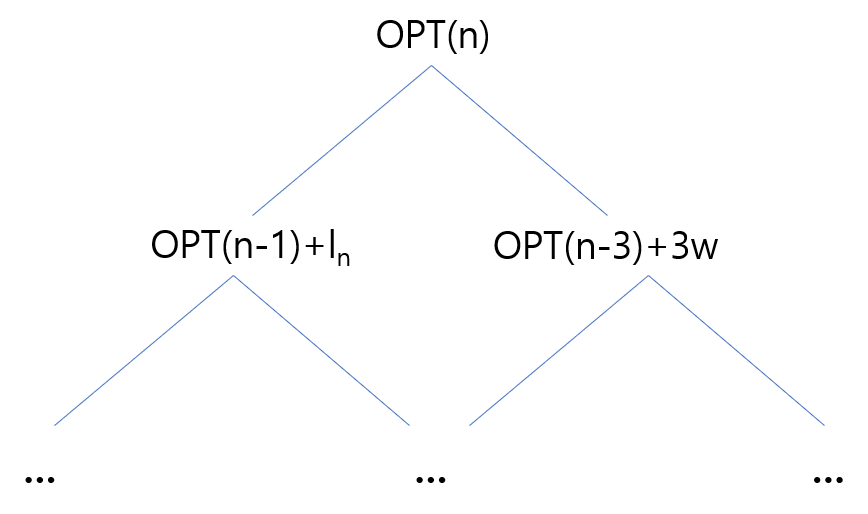
\includegraphics[scale=0.5]{figure1.png}
	\caption{Tree of the subproblem}
\end{figure}

But this method will result in exponential time complexity. So we use memoization to make it faster. Following is my algorithm.

\[
  OPT(i) = \left.
  \begin{cases}
    0 & \text{for } i = 0 \\
    l_i r & \text{for } i = 1 \\
    l_{i-1} r + l_i  r & \text{for } i =2 \\
    \text{min}(OPT(i-1)+l_ir, OPT(i-3) + 3w)  & \text{for } i \geq 3
  \end{cases}
  \right\} 
\]
Above algorithm is used from iterating $i=0$ to $i=n$. For $i \geq 3$, after each $OPT(i)$  is calculated, the last job $i$ is either in last laundry job of block which uses $L_2$ or just in $L_1$. So the algorithm outputs correct answer.

{\bf Tracing}

Make a array $A$ of size n+1 which has all value as 1.
In the algorithm, each time ${min}(OPT(i-1)+l_ir, OPT(i-3) + 3w)$ chooses $OPT(i-3) + 3w$, change the $A[i-2],A[i-1],A$[i] to 2. After n iteration, the array holds the answer except for A[0], which means nothing.

{\bf Complexity}

The complexity of this algorithm is only $O(n)$. Because we use memoization, looking back costs constant time so each iteration will cost only O(1). Making array for tracing is also O(1).
\end{enumerate}



\end{document}
